\EnglishSourceFrame{GELFAND-P001415}{unlabelled}
(15) \underline{Theorem}. Let $\lambda$ be a diagram with $N$ elements and
$q\ne\sqrt[m]{1}$. Then $S_{\lambda}^{(k)}$ define a representation of the Hecke algebra
(in the generators $e_k$).

We shall construct the functions $W$.
$W_{-r}(\tau)$ for $r=1,2,\ldots$ are defined by the relations
\begin{equation}
 W_{-(r+1)}(\tau)=1-\frac{\tau}{W_{-r}(\tau)},\qquad r\geq0,
 \tag{16}
\end{equation}
[Crossed out: \EnglishUnclear{GELFAND-P001415}{eq16-cancelled}{and for $r\ne0$; possibly $r\geq0$.}]
\begin{equation}
 W_r(\tau)=1-W_{-r}(\tau),\qquad r\geq0;
 \tag{17}
\end{equation}

Or:

$W_{-r}(\tau)$ is defined
[Crossed out: \EnglishUnclear{GELFAND-P001415}{continued-fraction-cancelled-word}{illegible}]
by the continued-fraction expansion:
\begin{equation}
 \text{[Crossed out: }W_{-r}(\tau)=\text{]}\quad
 1-\frac{\tau}{1-\dfrac{\tau}{1-\ldots}}
 \tag{18}
\end{equation}
There is the equation:
\begin{equation}
 W_r(\tau)W_{1-r}(\tau)=1.
 \tag{19}
\end{equation}
\EnglishUnclear{GELFAND-P001415}{eq19-right-hand-side}{The right side is written as $1$.}

General formula:
\begin{equation}
 W_r(\tau)=\frac{q(q^{r-1}-1)}{(q+1)(q^r-1)},\qquad r=1,2,\ldots
 \tag{20}
\end{equation}
\begin{equation}
 W_{-r}(\tau)=\frac{q^{r+1}-1}{(q+1)(q^r-1)}.
 \tag{21}
\end{equation}
\EnglishUnclear{GELFAND-P001415}{w-index}{The index of the functions $W$ is $r$; possibly $i$.}

(22) \underline{Problem}: find the characters of the Hecke algebra.

Consider
\begin{equation}
 \frac{
 \begin{vmatrix}
 x_1^{i_1}&x_1^{i_2+1}&\ldots&x_1^{i_n+n-1}\\
 x_2^{i_1}&x_2^{i_2+1}&\ldots&x_2^{i_n+n-1}\\
 \ldots&\ldots&\ldots&\ldots\\
 x_n^{i_1}&\ldots&\ldots&x_n^{i_n+n-1}
 \end{vmatrix}
 }{
 \begin{vmatrix}
 1&x_1&x_1^2&\ldots&x_1^{n-1}\\
 1&x_2&x_2^2&\ldots&\\
 \ldots&\ldots&\ldots&\ldots&\\
 1&x_n&x_n^2&\ldots&x_n^{n-1}
 \end{vmatrix}
 }
 =\sum a(i,j)P_{j_1}P_{j_2}\ldots P_{j_n}
 \tag{23}
\end{equation}
\EnglishUnclear{GELFAND-P001415}{eq23-overwritten-exponents}{In the first two rows of the numerator's last column: $i_n+n-1$; the subscript of $i$ is corrected over earlier strokes.}


\EnglishSourceFrame{GELFAND-P001416}{53}
$j=(j_1,\ldots,j_n)$, $P_j$ is a power sum.

Then

(24) $a(i,j)$ is the value of a character [inserted above the line: of the symmetric group]
on an element with cycle lengths $j_1,\ldots,j_n$

(up to a simple constant)

For the symmetric group, see Macdonald's book, “Symmetric functions
and Hall polynomials”.

\medskip
\underline{Location of the poles of the Ruelle zeta function.}

(\EnglishUnclear{GELFAND-P001416}{mayer-name}{Lindon Mayer (?) [source candidate]})

Letters in Math. Physics, $14:2$, 1987

$I$ is an interval; $T:I\to I$ is piecewise linear
\begin{equation*}
 I=\bigcup_j I_j,\qquad T(I_j)=I.
\end{equation*}
\EnglishSourceFigure{GELFAND-P001416}{interval-graph}{An unlabelled rectangular frame contains several ascending slanted branches and nearly vertical strokes. Which branches the short strokes belong to, and the exact number of discontinuities, require comparison with the original.}

\begin{center}
\begin{minipage}[t]{.46\linewidth}\vspace{0pt}\centering
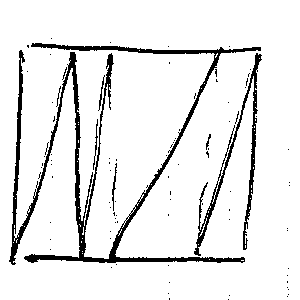
\includegraphics[width=\linewidth]{figures/gelfand-0154-p001416-interval-graph-original.png}\par\smallskip
{\footnotesize Original manuscript detail: \texttt{GELFAND-P001416}}
\end{minipage}\hfill
\begin{minipage}[t]{.50\linewidth}\vspace{0pt}\centering
{\footnotesize Partial visible-stroke recreation}\par\smallskip
\resizebox{\linewidth}{!}{% Visible strokes only. Coordinate scale reproduces the sketch, not an exact map.
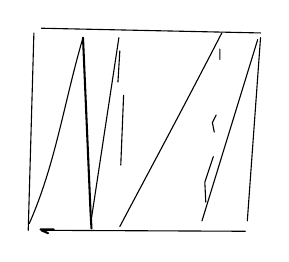
\begin{tikzpicture}[x=.012cm,y=-.012cm,line cap=round]
\draw (20,50)--(14,259) (28,45)--(260,50) (260,55)--(246,249)
 (31,259)--(244,260);
\draw (15,252) .. controls (43,189) and (52,123) .. (72,55);
\draw[line width=.75pt] (72,55)--(80,240)--(81,257);
\draw (81,246)--(110,55);
\draw (111,69)--(109,102) (115,116)--(112,190);
\draw (111,255) .. controls (140,200) and (171,143) .. (219,50);
\draw (198,249)--(257,57);
\draw (202,229)--(201,208)--(210,181) (211,155)--(209,145)--(213,137)
 (217,67)--(217,78);
% The thick bottom-left terminal trace is not interpreted as an arrow.
\draw[line width=.75pt] (27,258)--(41,258) (28,259)--(35,262);
\end{tikzpicture}
}
\end{minipage}
\end{center}
\noindent{\small\textit{Open joins and short vertical traces remain unresolved after 3×, 5× and 10× inspection. Plain strokes do not specify arrows, discontinuities or extra axis values.}}


\begin{equation}
 \zeta_T(z,\varphi)=\frac{\det(1-zL_1)}{\det(1-zL_2)},
 \tag{1}
\end{equation}
where
\begin{equation*}
 L_1f(z)=\varphi(z)\sum\frac{1}{\rho_j}f(\psi_j(z)),
\end{equation*}
\begin{equation*}
 L_2f(z)=\varphi(z)\sum f(\psi_j(z)),
\end{equation*}
$\psi_j$ are local inverses of $T$ on the interval $I_j$, and $\rho_j^{-1}$ is the slope.
\EnglishUnclear{GELFAND-P001416}{slope-letter}{The letter in $\rho_j$ also admits the reading $p_j$.}

In the general case:
\begin{equation}
 \zeta_T(z,\varphi)=
 \exp\left(
 \sum_{n=1}^{\infty}\frac{z^n}{n}
 \sum_{\xi\in\mathrm{Fix}\,T^n}
 \prod_{k=0}^{n-1}\varphi(T^k x)
 \right)
 \tag{2}
\end{equation}
\EnglishUnclear{GELFAND-P001416}{eq2-variable}{Below the second sum is written $\xi\in\mathrm{Fix}\,T^n$; in the product, $x$.}


\EnglishSourceFrame{GELFAND-P001417}{unlabelled}
\underline{7/XII-87.}\qquad \underline{Gelfand seminar!}\qquad Something on the paper by

\underline{D. Mayer}\qquad \underline{Lett. in Math. Phys. 1987, $14:2$}

\underline{On the Ruelle $\zeta$ function}

$F$ is the set of spin values (finite).

We study spin configurations on a lattice
\begin{equation*}
 (\xi_i),\qquad -\infty<i<\infty,\qquad \xi_i\in F.
\end{equation*}
$M\subseteq F\times F$ is the admissible set; we require
\begin{equation}
 (\xi_i,\xi_{i+1})\in M.
 \tag{1}
\end{equation}

The simplest example of a Ruelle $\zeta$ function is the Artin–Mazur $\zeta$ function.

Consider the set of periodic configurations and their number:
\begin{equation}
 N_n=\#\{(\xi_i)\mid\mathcal T^n(\xi_i)=(\xi_i)\}
 =\mathrm{Fix}\,\mathcal T^n,
 \tag{2}
\end{equation}
where $\mathcal T$ is the transformation in the sequence space
\begin{equation*}
 \mathcal T(\xi_i)=\xi_{i+1}
\end{equation*}
(shift)

The Ruelle $\zeta$ function:
\begin{equation}
 \zeta_{\mathcal T}(s)=\exp\left(\sum_{n=1}^{\infty}\frac{N_n}{n}s^n\right)
 \tag{3}
\end{equation}
the series converges for $|s|<\dfrac{1}{|F|}$.

\EnglishUnclear{GELFAND-P001417}{continuation-question-overwriting}{Does analytic continuation exist? [The end of the source abbreviation “Sushch.” and the initial “a” are retraced over earlier strokes.]}
Consider the matrix
\begin{equation}
 T=(T_{\alpha\beta})=
 \begin{cases}
 1,&(\alpha,\beta)\in M,\\
 0,&(\alpha,\beta)\notin M.
 \end{cases}
 \tag{4}
\end{equation}

Then
\begin{equation}
 \zeta_{\mathcal T}(s)=\frac{1}{\det(1-sT)}
 \tag{5}
\end{equation}

It follows that $\zeta_{\mathcal T}(s)$ is meromorphic.

The radius of convergence may exceed $1/|F|$.

For the proof, note that
\begin{equation}
 N_n=\mathrm{Tr}\,T^n.
 \tag{6}
\end{equation}


\EnglishSourceFrame{GELFAND-P001418}{62}
\underline{Remark by I. M. G.}: this resembles the work of Dynkin and Dmitriev:
consider a stoch. matrix $(p_{ik})$ [inserted above: (stochastic)]
(in the problem of reservoirs, this is
[crossed-out sign: \EnglishUnclear{GELFAND-P001418}{basin-cancelled-sign}{illegible}]
the fraction of water flowing from reservoir $i$ into reservoir $k$).
\begin{equation*}
 \underline{P}=(p_{ik}),\qquad \sum_k p_{ik}=1.
\end{equation*}
This depends on the eigenvalues of $P$.

a) The eigenvalues lie in the disk $|\lambda|\leq1$,

b) $1$ is an eigenvalue.

What region do the eigenvalues fill?

It is the interior of some algebraic curve.

They did it incorrectly.

There is a family of eigenvalues!!

and one should draw the family of eigenvalues in $\mathbb C^n$---it should
be a beautiful region (\underline{Problem!!})

Projection onto one axis may be complicated!

[A double line on the left; the following two lines are underlined:]
\underline{In the Ruelle problem, it is interesting to examine all eigenvalues}

\underline{of the matrix $T$.}

\medskip
\underline{Speaker}. Generalisation of example (3)
\begin{equation}
 \zeta_{\mathcal T}(s;\varphi)=
 \exp\left(
 \sum_{n=1}^{\infty}\frac{s^n}{n}
 \sum_{\xi\in\mathrm{Fix}(\mathcal T^n)}
 \prod_{\ell=0}^{n}\varphi(\mathcal T^\ell\xi)
 \right)
 \tag{7}
\end{equation}
\EnglishUnclear{GELFAND-P001418}{eq7-upper-product-bound}{The upper product limit is written as $n$.}

Here
\begin{equation*}
 \varphi=\varphi(\xi_1,\ldots,\xi_k),\qquad \xi_j\in F
\end{equation*}
[Below $\varphi$, a line leads to the caption: function.]

($\varphi$ depends only on the first $k$ values).

((3) is obtained for $\varphi=1$)

(8) \underline{Assertion.} $\exists$ [crossed out: operator; inserted above the line: matrix]
$L$ (finite-dimensional), such that:
\begin{equation}
 \zeta_{\mathcal T}(s,\varphi)=\frac{1}{\det(1-sL)}
 \tag{9}
\end{equation}

Specifically, consider
\begin{equation*}
 F'=F^k;
\end{equation*}
[Crossed out: \EnglishUnclear{GELFAND-P001418}{before-m-prime-cancelled}{an illegible entry before $M'$}.]
\begin{equation*}
 M'\subset F'\times F'
\end{equation*}
\begin{equation}
 M'=\{(\xi_1,\ldots,\xi_k);(\xi_2,\ldots,\xi_{k+1})
 \mid(\xi_i,\xi_{i+1})\in M\}
 \tag{10}
\end{equation}
\EnglishUnclear{GELFAND-P001418}{eq10-overwritten-indices}{In the second tuple, the indices $2$ and $k+1$ are corrected; in the condition, $i+1$ is also retraced.}

Then take
\begin{equation*}
 \ell_{\alpha\beta}=
 \begin{cases}
 \varphi(\alpha),&(\alpha,\beta)\in M',\\
 0,&(\alpha,\beta)\notin M',
 \end{cases}
 \qquad L=(\ell_{\alpha\beta}).
\end{equation*}


\EnglishSourceFrame{GELFAND-P001419}{unlabelled}
\underline{I. M. G.:}

\underline{NB}: one must know the $p$-adic numbers

(be able to add, multiply and divide them,
[crossed out: \EnglishUnclear{GELFAND-P001419}{nb-cancelled-letter}{an illegible sign}]
extract roots!)

\medskip
\underline{A. Beilinson}\qquad
\underline{$p$-adic numbers and physics.}

\underline{On some of Manin's $p$-adic ideas in physics}
\EnglishUnclear{GELFAND-P001419}{heading-last-sign}{!; possibly ?}

$1^{\circ}$. Witten listened to a talk by
\EnglishUnclear{GELFAND-P001419}{faltings-name}{Faltins [source candidate]}
with great interest, after which he bought all the books on number theory.
The only thing he understood from the talk was the formula
\begin{equation}
 |a|_\infty\cdot|a|_2|a|_3\ldots=1,\qquad a\in\mathbb Q.
 \tag{1}
\end{equation}
For $\dfrac12$, this reads:
\begin{equation*}
 \frac12\cdot2\cdot1\ldots=1.
\end{equation*}

There are three papers:

1) \underline{Volovich}\qquad (in Russian)

2) \underline{Yu. I. Manin}\qquad (in English)

3) \underline{Witten} and someone else
\EnglishUnclear{GELFAND-P001419}{witten-list-final-sign}{[an illegible separate sign after the line]}

All three papers appeared in September.

\underline{Witten's text.}

Consider the functional equation for the Riemann $\zeta$ function
\begin{equation}
 \pi^{-s/2}\Gamma(s/2)\prod(1-p^{-s})^{-1}
 =
 \pi^{-(1-s)/2}\Gamma\left(\frac{1-s}{2}\right)
 \prod(1-p^{-(1-s)})^{-1}.
 \tag{2}
\end{equation}
(analytic continuation is understood)

or (formally):
\begin{equation}
 \frac{\pi^{-s+1}\Gamma(s/2)}
 {\Gamma\left(\dfrac{1-s}{2}\right)}
 =
 \prod_p\frac{1-p^{-s}}{1-p^{s-1}}.
 \tag{3}
\end{equation}
\EnglishUnclear{GELFAND-P001419}{eq3-pi-exponent}{The exponent of $\pi$ is written as $-s+1$.}

On the left is $\approx$ the Veneziano–Witten amplitude for an open
string [inserted above: (with momentum $s$)].
On the right is a divergent expression, but what matters is
that it is represented as a product over the primes!


\EnglishSourceFrame{GELFAND-P001420}{63}
\underline{$2^{\circ}$. On Manin's work}

(1) \underline{Assertion}: The Tamagawa measure $=1$.

In more detail:
\begin{equation*}
 \mathrm{SL}(n,\mathbb R)\supset\mathrm{SL}(n,\mathbb Z).
\end{equation*}
On $\mathrm{SL}(n,\mathbb R)$ there is an invariant measure (standard)
[above “invariant”, inserted: left].

Normalise [crossed out:
\EnglishUnclear{GELFAND-P001420}{normalization-cancelled}{illegible}]
using the integer matrices.
\begin{equation*}
 \operatorname{vol}\bigl(\mathrm{SL}(n,\mathbb R)/\mathrm{SL}(n,\mathbb Z)\bigr)-?
\end{equation*}

[In the right margin:]
(constructed using the standard basis in the Lie algebra
$\mathfrak{sl}(n,\mathbb R)$ or in $\mathfrak{gl}(n,\mathbb R)$
[crossed out: \EnglishUnclear{GELFAND-P001420}{margin-cancelled}{an illegible sign}]
standard basis;
\begin{center}
 \fbox{$\operatorname{vol}_{sl}=\dfrac{\operatorname{vol}_{gl}}{d\,\operatorname{tr}}$}
\end{center}
\EnglishUnclear{GELFAND-P001420}{margin-volume-formula}{The marginal formula: $\operatorname{vol}_{sl}=\operatorname{vol}_{gl}/d\,\operatorname{tr}$; the small letters beside $\operatorname{vol}$ require checking.}

$\mathrm{SL}(2,\mathbb R)$ consists of conformal transformations of the unit disk, acting transitively
on $S^*H^2$.

The invariant volume on $S^*H^2$ is
[crossed out: \EnglishUnclear{GELFAND-P001420}{invariant-volume-cancelled}{an illegible sign}]
$\operatorname{vol}_{H^2}\otimes d\varphi$.

\begin{center}
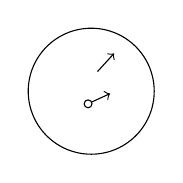
\begin{tikzpicture}[x=1cm,y=1cm]
 \draw (0,0) circle (0.8);
 \draw (-0.04,-0.16) circle (0.05);
 \draw[->] (0,-0.14) -- (0.24,-0.03);
 \draw[->] (0.08,0.25) -- (0.29,0.48);
\end{tikzpicture}
\end{center}

Or: quotient by the maximal compact subgroup

\begin{center}
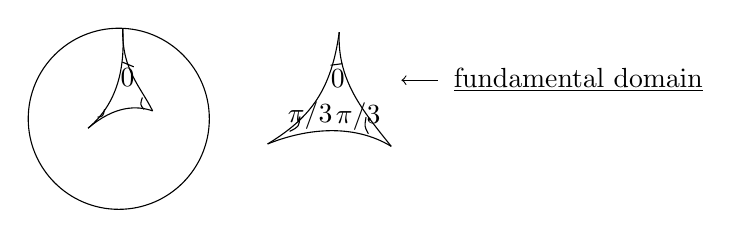
\begin{tikzpicture}[x=1cm,y=1cm]
 \draw (0,0) circle (1.15);
 \draw (0.05,1.14) .. controls (0.08,0.65) and (-0.01,0.2) .. (-0.39,-0.12);
 \draw (0.05,1.14) .. controls (0.04,0.62) and (0.27,0.42) .. (0.43,0.10);
 \draw (-0.39,-0.12) .. controls (-0.05,0.17) and (0.23,0.17) .. (0.43,0.10);
 \draw (0.045,0.72) -- (0.19,0.66);
 \draw (-0.27,0.02) .. controls (-0.2,0.03) .. (-0.18,0.12);
 \draw (0.32,0.12) .. controls (0.27,0.18) .. (0.30,0.27);
 \node at (0.11,0.52) {$0$};
 \draw (2.8,1.1) .. controls (2.7,0.38) and (2.45,0.02) .. (1.89,-0.32);
 \draw (2.8,1.1) .. controls (2.77,0.48) and (3.11,0.09) .. (3.46,-0.35);
 \draw (1.89,-0.32) .. controls (2.39,-0.12) and (2.98,-0.06) .. (3.46,-0.35);
 \draw (2.69,0.68) -- (2.84,0.7);
 \draw (2.17,-0.16) .. controls (2.29,-0.1) .. (2.30,0.03);
 \draw (3.17,-0.19) .. controls (3.12,-0.10) .. (3.14,0.02);
 \node at (2.78,0.51) {$0$};
 \node at (2.43,0.04) {$\pi/3$};
 \node at (3.04,0.03) {$\pi/3$};
 \draw[->] (4.05,0.49) -- (3.59,0.49);
 \node[anchor=west] at (4.13,0.49) {\underline{fundamental domain}};
\end{tikzpicture}
\end{center}

\underline{Answer.}
\begin{equation}
 \operatorname{vol}\mathrm{SL}(n,\mathbb R)/\mathrm{SL}(n,\mathbb Z)
 =\zeta(2)\zeta(3)\ldots\zeta(n)
 \tag{2}
\end{equation}
$\mathbb A$ denotes the adeles;
\begin{equation}
 \begin{gathered}
 \mathrm{SL}(n,\mathbb A)\sim
 \mathrm{SL}(n,\mathbb R)\times\mathrm{SL}(n,\mathbb Q_2)\times\ldots\\
 \cup\\
 \mathrm{SL}(n,\mathbb Q)
 \end{gathered}
 \tag{3}
\end{equation}
\begin{equation}
 \operatorname{vol}\mathrm{SL}(n,\mathbb A)/\mathrm{SL}(n,\mathbb Q)=1.
 \tag{4}
\end{equation}
\begin{equation*}
 \operatorname{vol}\mathrm{SL}(n,\mathbb A)/\mathrm{SL}(n,\mathbb Q)
 \sim
 \operatorname{vol}\mathrm{SL}(n,\mathbb R)/\mathrm{SL}(n,\mathbb Z)
 \prod\operatorname{vol}\mathrm{SL}(n,\mathbb Z_p).
\end{equation*}
\begin{equation}
 \operatorname{vol}\mathrm{SL}(n,\mathbb Z_p)
 \sim\#\mathrm{SL}_n(\mathbb F_p)/p^{n^2-1}.
 \tag{5}
\end{equation}
\underline{Exercise}: calculate $\#\mathrm{SL}_n(\mathbb F_p)$.


\EnglishSourceFrame{GELFAND-P001421}{unlabelled}
(6) The number of elements of $\mathrm{GL}(n,\mathbb F_p)$
\begin{equation*}
 (p^n-1)(p^n-p)(p^n-p^2)\ldots
 =
 p^{n^2}(1-p^{-n})(1-p^{-n+1})\ldots(1-p^{-1}).
\end{equation*}

(7) For $\mathrm{SL}(n,\mathbb F_p)$, divide by $p-1$:
\begin{equation*}
 p^{n^2-1}(1-p^{-n})(1-p^{-n+1})\ldots(1-p^{-2}).
\end{equation*}
This is a product of Euler factors.

(8) \underline{Conjecture of Yu. I. Manin}: an analogue of formula (2) can be written for
the moduli spaces of curves arising in string theory.

\underline{I. M. G.}

\underline{Mathematical question}: the volume of Teichmüller space has a $p$-adic analogue.

Or: what is adelic Teichmüller space

\medskip
\underline{An example of the \EnglishUnclear{GELFAND-P001421}{witten-heading-faint-word}{power} of Witten's work:}

\underline{Laumon} produced a work in number theory based on Witten's ideas
from Morse theory.

Idea: consider a function $u\in\mathcal E'(\mathbb R)$,
$\widetilde u(\xi)\in C^\infty$
and all singularities will move into the asymptotics at infinity.

\underline{Advice from I. M. G.}: read Kharkevich's book
“Spectra, [crossed out:
\EnglishUnclear{GELFAND-P001421}{book-title-cancelled}{illegible};
inserted above the line: signals] and noise”,
to understand the \underline{Fourier transform}.

On the work of \underline{Laumon}.

\begin{center}
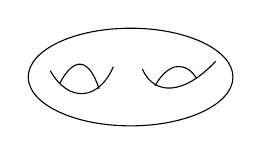
\begin{tikzpicture}[x=1cm,y=1cm]
 \draw (0,0) ellipse (1.3 and 0.62);
 \draw (-1.02,0.08) .. controls (-0.78,-0.34) and (-0.40,-0.29) .. (-0.22,0.13);
 \draw (-0.90,-0.08) .. controls (-0.72,0.26) and (-0.53,0.25) .. (-0.40,-0.15);
 \draw (0.15,0.10) .. controls (0.30,-0.24) and (0.68,-0.23) .. (1.08,0.20);
 \draw (0.31,-0.11) .. controls (0.50,0.22) and (0.72,0.18) .. (0.84,-0.02);
\end{tikzpicture}
\end{center}

Consider the surface $\mathcal F$
\begin{equation*}
 H^i(X,\mathcal F),\qquad i=0,1,2.
\end{equation*}
\EnglishUnclear{GELFAND-P001421}{surface-symbol}{After “surface” is written $\mathcal F$; subsequently, $H^i(X,\mathcal F)$.}

\begin{equation}
 \det H^\bullet(X,\mathcal F)=
 \frac{\det H^0(X,\mathcal F)\det H^2(X,\mathcal F)}
 {\det H^1(X,\mathcal F)\;
 \text{[crossed out: }\det H^2(X,\mathcal F)\text{]}}
 \tag{1}
\end{equation}
([Crossed out:
\EnglishUnclear{GELFAND-P001421}{before-vector-spaces-cancelled}{finite?}]
vector spaces;
$\det$ is the highest exterior power)

Automorphisms?

Consider a triangulation; $\det H^\bullet$ is identified with the product of the $\det$
of the terms of the complex (an Euler-type formula): canonically


\EnglishSourceFrame{GELFAND-P001422}{64}
\begin{equation*}
\det(C^\bullet)=\det(H^\bullet(C)) \tag{2}
\end{equation*}
$2-2g$ is the Euler characteristic.

On the other hand
\begin{equation*}
2g-2=\operatorname{deg}K
\end{equation*}
[Below $K$: “canonical class”.]

\underline{Let}

$D$ be a divisor;
\begin{equation*}
\det\mathcal F_D=\bigotimes(\det\mathcal F_{x_i})^{\otimes a_i},
\qquad D=\sum a_i x_i \tag{3}
\end{equation*}
[Crossed out:
\EnglishUnclear{GELFAND-P001422}{cancelled-divisor-map}{$D\to D+K$ or $D\mapsto D+K$; reading not established}.]

\underline{Deligne's formula:}
\begin{equation*}
\det H^\bullet=\det\mathcal F_K \tag{4}
\end{equation*}
[A separate sign on the right is crossed out:
\EnglishUnclear{GELFAND-P001422}{eq4-cancelled-sign}{illegible}.]
\EnglishUnclear{GELFAND-P001422}{eq4-determinant-convention}{In (4), $\det H^\bullet=\det\mathcal F_K$ is written without an exponent $-1$.}

(fix a complex structure and a choice of point in the canonical class)

For an arbitrary constructible sheaf, $\underline{\det}$ is also defined, and
there is an analogue of Deligne's formula!

Here functions with singularities arise on $\mathbb A^1$

\underline{\underline{Klyachko.}}\quad
\underline{\underline{Toric bundles.}}

A toric variety is a variety $X$ on which an algebraic torus $T$ acts;
there is an orbit isomorphic to $T$.
\begin{equation*}
X=\bigcup_\sigma O_\sigma,\quad\text{--- decomposition into orbits}
\end{equation*}
$\mathcal E$ is a bundle on $X$ with a toric structure
(and the action lifts! The diagram
\begin{equation*}
\begin{tikzcd}
\mathcal E \arrow[r,"t"] \arrow[d] & \mathcal E \arrow[d] \\
X \arrow[r,"t"] & X
\end{tikzcd}
\end{equation*}
commutes)

One can describe the moduli of [inserted above the line: “such”]
bundles in the language of linear algebra.


\EnglishSourceFrame{GELFAND-P001423}{unlabelled}
The structure of $X$ is described by a fan $\Sigma$ in the Lie algebra of the torus.
\begin{center}
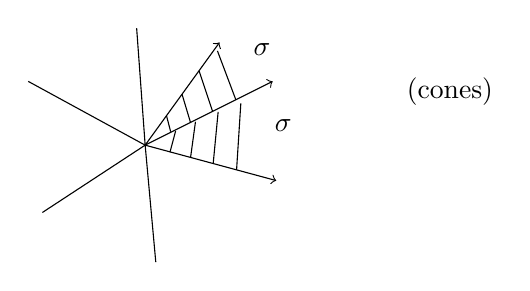
\begin{tikzpicture}[scale=0.9]
\draw (0,0) -- (-1.65,0.9);
\draw (0,0) -- (-1.45,-0.95);
\draw (0,0) -- (-0.12,1.65);
\draw (0,0) -- (0.15,-1.65);
\draw[->] (0,0) -- (1.05,1.45);
\draw[->] (0,0) -- (1.8,0.9);
\draw[->] (0,0) -- (1.85,-0.5);
\draw (0.36,0.19) -- (0.3,0.42);
\draw (0.64,0.32) -- (0.52,0.72);
\draw (0.95,0.48) -- (0.76,1.05);
\draw (1.28,0.64) -- (1.02,1.33);
\draw (0.35,-0.10) -- (0.43,0.20);
\draw (0.64,-0.18) -- (0.71,0.33);
\draw (0.96,-0.26) -- (1.03,0.47);
\draw (1.29,-0.35) -- (1.35,0.59);
\node at (1.65,1.35) {$\sigma$};
\node at (1.95,0.28) {$\sigma$};
\node at (4.3,0.75) {(cones)};
\end{tikzpicture}
\end{center}
$|\Sigma|$ is the set of $1$-dimensional cones of the fan $\Sigma$.

\underline{Theorem.}
(category of toric bundles) $\Longleftrightarrow$
(category of vector spaces
[crossed-out sign:
\EnglishUnclear{GELFAND-P001423}{theorem-cancelled-sign}{illegible}]
$E$ with a family [inserted above the line: “decreasing $\mathbb Z$-”]
of filtrations $E^\alpha(i)$, $\alpha\in|\Sigma|$, satisfying the condition

A) The filtrations $E^\alpha$, $\alpha\in\sigma\in\Sigma$,
are distributive.

\underline{Problems.}
1) Describe the geometry of the bundle (cohomology, characteristic classes
and so on) in terms of the filtrations

2) classification---?

Let $\Sigma$ be a simplicial complex; associate a filtration
to each vertex

A representation of it is a family of filtrations in a vector space
[inserted above the line: «$E$:»] $E^\alpha(i)$,
$\alpha\in$ [crossed-out sign:
\EnglishUnclear{GELFAND-P001423}{representation-cancelled-sign}{illegible}]
$\Sigma$,
\begin{equation*}
E\ldots\supset E^\alpha(i)\supset E^\alpha(i+1)\supset\ldots 0
\end{equation*}
\begin{equation*}
\alpha\in(\text{vertices of the complex})=\Sigma.
\end{equation*}
The spaces $E^\alpha(i)$, $\alpha\in\sigma$, are distributive for fixed $\sigma$
(for all $i$)

[Below the first $\sigma$: “simplex”. A framed insertion:]
(i.e. generate a distributive lattice)

For example, if

$\alpha_1,\alpha_2,\alpha_3$ are the vertices of a triangle $\Delta$, then

$E^{\alpha_1}\quad E^{\alpha_2}\quad E^{\alpha_3}$ are distributive, i.e.
\begin{equation*}
(E^{\alpha_1}+E^{\alpha_2})\cap E^{\alpha_3}
=E^{\alpha_1}\cap E^{\alpha_3}+E^{\alpha_2}\cap E^{\alpha_3}
\end{equation*}

\underline{Classify:} a good problem

For a triangle: it is solved trivially

For the surface of a tetrahedron $\Sigma=\partial\Delta$, where $\Delta$ is a simplex, the answer
is as follows: in [crossed out:
\EnglishUnclear{GELFAND-P001423}{tetrahedron-cancelled-space}{$\mathbb R^3$-space; reading not established}]
$E$, $\dim E=3$, consider $4$ $2$-dimensional subspaces in general position.
\begin{equation*}
\mathcal E=(E;\ E^\alpha,E^\beta,E^\gamma,E^\delta)
\end{equation*}


\EnglishSourceFrame{GELFAND-P001424}{65}
one must also take the exterior powers
\begin{equation*}
\Lambda^i\mathcal E=
(\Lambda^i E,\Lambda^i E^\alpha,\Lambda^i E^\beta,
\Lambda^i E^\gamma,\Lambda^i E^\delta)
\end{equation*}
A general representation decomposes into a direct sum of $1$-dimensional ones and these.

\underline{I. M. G.}
The right problem: isolate solvable parts in $\forall$ problem
(the Gelf.–Ponomarev approach)

V. [a corrected and crossed-out initial:
\EnglishUnclear{GELFAND-P001424}{kac-initial}{illegible}]
\underline{Kac} describes all this in the language of graphs and
\underline{Kac–Moody algebras}:
the dimensions at the vertices = coordinates of roots, and so on.

The number of parameters is found.

Lect. Notes, \underline{996}; an earlier paper — \underline{Inventiones}.

(a conference talk)

[A line is crossed out:
\EnglishUnclear{GELFAND-P001424}{cancelled-seminar-line}{Seminar \ldots; the rest is illegible}.]

\EnglishIncomplete{GELFAND-P001424}{cancelled-seminar-content}{A full reading of the crossed-out line before “Next time: 8 February” has not been established; the possible initial word is given above.}

\underline{Next time:}\quad \underline{8 February.}

